\chapter{Scenarios}

\section{Scenario Rashidi}
Rashidi listens to Jazz on the radio. He really likes Louis Armstrong and wants to look up more information about him. He uses \textit{Google} to look up information about him and gets to the ArticlePlaceholder on Hausa Wikipedia. There he can read up his date of birth (\textit{4 August 1901}), his place of birth (\textit{New Orleans}) \citep{wd:03} and get more information on, for example, New Orleans and learn, that New Orleans is a city in the United States of America. 
\begin{figure}[H]
	\centering
	\includegraphics[width=\textwidth]{diagrams/UserDiagramRashidiArmstrong.png}
	\caption{Scenario Rashidi}
	\label{fig:ScenarioRashidi}
\end{figure}

\section{Scenario Edha} 
Edha talks with friends about an exhibition they have been to. She hears about Rembrandt, a Dutch painter. As soon as she comes home, she realizes, she forgot to ask which century he lived in and where in the Netherlands he was born. She wants to look up the information on Wikipedia in her language. \\
\\ 
She opens Wikipedia and enters ``Rembrandt'' in the searchbar. Since there is no article on Rembrandt yet, she finds the ArticlePlaceholder for \textit{``Rembrandt'' (Q5598)} \citep{wd:01} in the result page. Since it also displays the description of the item (\textit{Dutch 17th century painter and etcher}) on the search page next to the name of the painter, she can validate with that description that she found the right information. \\
She gets an overview of Rembrandt on the page and can find the place of birth on the ArticlePlaceholder, which is \textit{Leiden}. She does not know the place and searches for it on Wikipedia again. She finds the description \textit{city and municipality in South Holland, Netherlands} \citep{wd:02} on the search page already. That is the information she was looking for, so she goes back to the ArticlePlaceholder. Since in the meantime someone edited the item on Wikidata, she finds even more information on him on the ArticlePlaceholder now. It also tells her his date of birth is \textit{15 July 1606} \citep{wd:01}. \\
\\
In the next days, she researches more on Rembrandt in her local library. With this additional information she decides to create an article. She goes back to the ArticlePlaceholder to get some of the informations and references, that are already there. Then she clicks the button \textit{create an article}, which is labeled in her language. She is able to add the title for the page, which is translated \textit{Rembrandt (painter)} in English to make clear which Rembrandt she means. This title differs from the title of the ArticlePlaceholder, which is only \textit{Rembrandt}. She can enter the information she researched and create an actual article.
\begin{figure}[H]
	\centering
	\includegraphics[width=\textwidth]{diagrams/UserDiagramEdhaRembrandt.png}
	\caption{Scenario Edha}
	\label{fig:ScenarioEdha}
\end{figure}

\section{Scenario Julian}
When ArticlePlaceholder would be enabled on German Wikipedia Julian would hear about it \todo{Make sure it's understandable they are not actually enabled yet?}. Since this Wikipedia has quite a lot of articles, he is aware, that he rarely will need them. \\
As part of a presentation in school, he wants to research \textit{KDE e.V.}. He searches for it on Wikipedia and gets to the ArticlePlaceholder. He uses the references provided to the data there. \\
He dislikes the way the data is displayed though. Therefore he wants to adjust the layout. He has contributed to a module before, so he knows how to write Lua code. He wants to overwrite one of the functions. After having a discussion with the local community which supports Julian's changes, he adds the code after testing it and the ArticlePlaceholder is adjusted to the community's needs. 
\begin{figure}[H]
	\centering
	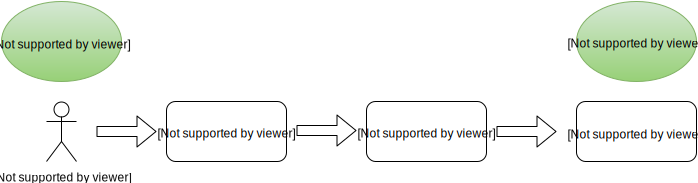
\includegraphics[width=\textwidth]{diagrams/UserDiagramJulianLua.png}
	\caption{Scenario Julian}
	\label{fig:ScenarioJulian}
\end{figure}

\section{Scenario Catrin}
One of Catrin's students tells her she used to live in \textit{Kasımpaşa}. She has never heard of it and back at home she wants to research it on French Wikipedia. She enters the term in the search bar. Since there is no article on the French Wikipedia, she gets to an ArticlePlaceholder. It does not have a description, so she can only see the name. She learns it is an \textit{instance of neighborhood} and is \textit{located in the administrative territorial entity Beyoğlu}. Since she has not heard of Beyoğlu yet either, she continues her research and gets to the French Wikipedia article Beyoğlu. There she finds out Beyoğlu is a district of Istanbul, Turkey.
\begin{figure}[H]
	\centering
	\includegraphics[width=\textwidth]{diagrams/UserDiagramCatrinKasimpase.png}
	\caption{Scenario Catrin}
	\label{fig:ScenarioCartin}
\end{figure}

\section{Scenario Heather}

Heather worked on the Wikidata item \textit{``Ada Lovelace'' (Q7259)} over the last days. She added data and mainly references by hand. She wants to see what the item looks like on a Wikipedia, that does not have an article on \textit{Ada Lovelace} yet. \\
She is involved with various small language Wikipedias and even though she does not speak the language, she can find the SpecialPage, which will bring her to an ArticlePlaceholder and enters the item ID there to see what it looks like. \\
When she enters the same item ID on English Wikipedia, she is redirected to the existing article on \textit{Ada Lovelace}.
\begin{figure}[H]
	\centering
	\includegraphics[width=\textwidth]{diagrams/UserDiagramHeatherSmallWP.png}
	\caption{Scenario Heater, small Wikipedia}
	\label{fig:ScenarioHeatherSmall}
\end{figure}
\begin{figure}[H]
	\centering
	\includegraphics[width=\textwidth]{diagrams/UserDiagramHeatherEnWiki.png}
	\caption{Scenario Heater, English Wikipedia}
	\label{fig:ScenarioHeatherEnWiki}
\end{figure}